\documentclass[12pt]{article}

\usepackage[spanish]{babel}
\usepackage[none]{hyphenat}
\usepackage[margin=3cm]{geometry}
\usepackage{enumitem}
\usepackage{longtable}
\usepackage{multirow, makecell}
\usepackage{listings}
\usepackage{color}
\usepackage{graphicx}
\usepackage{subcaption}
\usepackage{parskip}
\usepackage[hidelinks]{hyperref}

\definecolor{dkgreen}{rgb}{0,0.6,0}
\definecolor{gray}{rgb}{0.5,0.5,0.5}
\definecolor{mauve}{rgb}{0.58,0,0.82}

\lstset{
    language=Java,
    aboveskip=3mm,
    belowskip=3mm,
    showstringspaces=false,
    columns=flexible,
    basicstyle={\small\ttfamily},
    numbers=none,
    numberstyle=\tiny\color{gray},
    keywordstyle=\color{blue},
    commentstyle=\color{dkgreen},
    stringstyle=\color{mauve},
    breaklines=true,
    breakatwhitespace=true,
    tabsize=3
}

\sloppy
\setlength{\parindent}{0cm}
\decimalpoint
\graphicspath{{img/}}
\hypersetup{colorlinks=true, urlcolor=blue, citecolor=blue}
\urlstyle{same}

\begin{document}
    \begin{titlepage}
        \begin{center}
            \begin{figure}[ht]
                \centering
                \begin{subfigure}[r]{0.2\textwidth}
                    
\includegraphics[width=\textwidth]{Escudo_UNAM.png}
                \end{subfigure} \hspace{9cm}
                \begin{subfigure}[l]{0.2\textwidth}
                    
\includegraphics[width=\textwidth]{Escudo_FI.png}
                \end{subfigure} 
            \end{figure}

            \Huge \textbf{\\Laboratorio de Programación Orientada a Objetos\\}
            \huge\textbf{\\Práctica 1. Entorno y Lenguaje de Programación\\}
            \textbf{\\Profesor\\}
            \Large{M.C. Leonardo Ledesma Dominguez \\}
            \huge \textbf{\\Integrantes\\}
            \Large{Acosta Porcayo Alan Omar\\ Gutiérrez Grimaldo Alejandro\\Medina Villa Samuel}
        \end{center}
    \end{titlepage}

    \section*{Resumen}
    En esta práctica tendrá como objetivo familiarizarse y probar el entorno de ejecución y el lenguaje de programación java. Para ello se llevarán a cabo actividades para entender y experimentar los conceptos básicos del lenguaje de programación orientado a objetos, como clases, objetos, métodos y atributos, todo esto con el fin de resolver ciertos problemas empleando la sintaxis básica del lenguaje, incluyendo la notación adecuada, palabras reservadas y la incorporación de comentarios para documentar el código.

    \section*{Introducción}
    Introducción:
    Una comprensión completa de la programación orientada a objetos se logra al poner en práctica los conceptos teóricos en un lenguaje de programación real. En esta introducción, vamos a explorar los pasos clave para comenzar a programar en un lenguaje orientado a objetos. Abordaremos aspectos esenciales, como el entorno de trabajo, las herramientas disponibles y la importancia de practicar la programación para un aprendizaje efectivo.
    Explorando Java como Ejemplo de Lenguaje de Programación
    Un ejemplo práctico de lenguaje orientado a objetos es Java. Fue presentado por primera vez en 1995 por Sun Microsystems, que actualmente es propiedad de Oracle. Java se destaca por ser un lenguaje de alto nivel que combina elementos de los lenguajes C y C++. Sin embargo, lo que lo hace distintivo es su enfoque en la programación orientada a objetos. Una característica única de Java es su capacidad para ser compilado e interpretado, lo que lo convierte en una herramienta versátil para el desarrollo de software.

    \subsection*{El Mundo de Java: Plataforma y Estructura}
    El mundo de Java consta de dos componentes fundamentales: la JVM (Máquina Virtual Java) y la API (Interfaz de Programación de Aplicaciones Java). La JVM permite ejecutar programas Java al simular una ``máquina virtual'' independiente con su propio sistema operativo y hardware virtual. La API proporciona componentes predefinidos que hacen que el desarrollo y la implementación de aplicaciones sean más sencillos.
    
    \subsection*{Construyendo Programas en Java}
    En el contexto de Java, los programas se organizan en clases, que se escriben en archivos de texto con la extensión .java. Estos archivos luego se compilan en archivos binarios con extensión .class, que son independientes de la arquitectura. Durante la ejecución, la JVM interpreta los archivos .class y los traduce en instrucciones ejecutables para el sistema operativo.

    \subsection*{Herramientas de Desarrollo y Proceso de Compilación}
    Para el desarrollo en Java, el Java Development Kit (JDK) proporciona las herramientas esenciales. La compilación de archivos .java se realiza mediante el comando ``javac'' del JDK. Una vez compilado, el programa se puede ejecutar usando el comando ``java'', seguido por el nombre de la clase principal que contiene el método ``main()''.

    \subsection*{El Papel de los Entornos de Desarrollo Integrado (IDE)}
    Aunque es posible desarrollar programas utilizando un simple editor de texto y las herramientas del JDK, los Entornos de Desarrollo Integrado (IDE) ofrecen interfaces más amigables. Estos IDEs aprovechan las herramientas del JDK para simplificar y agilizar todas las etapas del desarrollo, desde escribir el código hasta ejecutarlo.
    
    \section*{Metodología} 

    \subsection*{Problema 1}
    Elabore un programa cuya salida sea:

    Cuando $m = 4$ ($m$ sea un numero par)
    \begin{figure}[h]
        
\includegraphics[width=2cm]{Cuadrado1.png}
    \end{figure}

    Cuando $m = 5$ ($m$ sea un numero impar)
    \begin{figure}[h]
        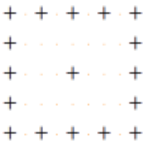
\includegraphics[width=3cm]{Cuadrado2.png}
    \end{figure}

    Donde $m$ es un número aleatorio entre 1 y 20, y cada número para imprime un cuadrado de base $m$ y cuando es impar de manera extra coloca el centro de la figura

    \hfil \break
    \textbf{Código}
    \begin{lstlisting}
codigo = false
    \end{lstlisting}

    \subsection*{Problema 2}
    Elabore un programa que reciba el del teclado un numero entero positivo mayor que 1, $k$ y realice un rombo cuya diagonal menor sea de tamaño $k$

    Ejemplo $k = 4$
    \begin{figure}[h]
        
\includegraphics[width=2cm]{Rombo.png}
    \end{figure}

    \hfil \break
    \textbf{Código}
    \begin{lstlisting}
codigo = false
    \end{lstlisting}

    \subsection*{Problema 3}
    Realice un programa que reciba de entrada (de tipo Scanner) de 2 a 6 números enteros positivos y determinar quién es el menor, el de en medio y el mayor. Los números que se reciban serán de uno a uno, ósea de manera secuencial.

    Ejemplo, se la entrada $\longrightarrow 4 ,2, 9, 100, 89, 3$
    
    \hfil \break
    Salida:
    
    \hfil \break
    Mayor: 100 \\
    Menor: 2 \\
    Mediana: 4

    \hfil \break
    \textbf{Código}
    \begin{lstlisting}
codigo = false
    \end{lstlisting}

    \subsection*{Problema 4}
    Programar ``War of Numbers'' el ejercicio de describe en: \\
    \url{https://edabit.com/challenge/7fHsizQrTLXsPWMyH}

    Sólo que, en lugar de recibir un arreglo de enteros, la guerra sea con 10 números aleatorios entre 1-1000

    \hfil \break
    \textbf{Código}
    \begin{lstlisting}
codigo = false
    \end{lstlisting}

    \subsection*{Problema 5}
    Programar el problema descrito en: \\
    \url{https://edabit.com/challenge/4r33Yd2HuEireb3Sm}

    \hfil \break
    \textbf{Código}
    \begin{lstlisting}
codigo = false
    \end{lstlisting}

    \section*{Resultados}

    \section*{Conclusiones}
    Al llevar a cabo esta práctica, hemos logrado reconocer los componentes fundamentales que conforman el lenguaje de programación Java. Estos elementos juegan un papel crucial en su funcionamiento y pertinencia en el ámbito de la programación. La colaboración entre estos conceptos, como la Máquina Virtual de Java (JVM), el Java Development Kit (JDK), la codificación y la compilación, sienta las bases en las cuales podemos edificar soluciones para desafíos tecnológicos.
\end{document}